\documentclass[]{article}
\usepackage{lmodern}
\usepackage{amssymb,amsmath}
\usepackage{ifxetex,ifluatex}
\usepackage{fixltx2e} % provides \textsubscript
\ifnum 0\ifxetex 1\fi\ifluatex 1\fi=0 % if pdftex
  \usepackage[T1]{fontenc}
  \usepackage[utf8]{inputenc}
\else % if luatex or xelatex
  \ifxetex
    \usepackage{mathspec}
  \else
    \usepackage{fontspec}
  \fi
  \defaultfontfeatures{Ligatures=TeX,Scale=MatchLowercase}
\fi
% use upquote if available, for straight quotes in verbatim environments
\IfFileExists{upquote.sty}{\usepackage{upquote}}{}
% use microtype if available
\IfFileExists{microtype.sty}{%
\usepackage{microtype}
\UseMicrotypeSet[protrusion]{basicmath} % disable protrusion for tt fonts
}{}
\usepackage[margin=1in]{geometry}
\usepackage{hyperref}
\hypersetup{unicode=true,
            pdfborder={0 0 0},
            breaklinks=true}
\urlstyle{same}  % don't use monospace font for urls
\usepackage{longtable,booktabs}
\usepackage{graphicx,grffile}
\makeatletter
\def\maxwidth{\ifdim\Gin@nat@width>\linewidth\linewidth\else\Gin@nat@width\fi}
\def\maxheight{\ifdim\Gin@nat@height>\textheight\textheight\else\Gin@nat@height\fi}
\makeatother
% Scale images if necessary, so that they will not overflow the page
% margins by default, and it is still possible to overwrite the defaults
% using explicit options in \includegraphics[width, height, ...]{}
\setkeys{Gin}{width=\maxwidth,height=\maxheight,keepaspectratio}
\IfFileExists{parskip.sty}{%
\usepackage{parskip}
}{% else
\setlength{\parindent}{0pt}
\setlength{\parskip}{6pt plus 2pt minus 1pt}
}
\setlength{\emergencystretch}{3em}  % prevent overfull lines
\providecommand{\tightlist}{%
  \setlength{\itemsep}{0pt}\setlength{\parskip}{0pt}}
\setcounter{secnumdepth}{0}
% Redefines (sub)paragraphs to behave more like sections
\ifx\paragraph\undefined\else
\let\oldparagraph\paragraph
\renewcommand{\paragraph}[1]{\oldparagraph{#1}\mbox{}}
\fi
\ifx\subparagraph\undefined\else
\let\oldsubparagraph\subparagraph
\renewcommand{\subparagraph}[1]{\oldsubparagraph{#1}\mbox{}}
\fi

%%% Use protect on footnotes to avoid problems with footnotes in titles
\let\rmarkdownfootnote\footnote%
\def\footnote{\protect\rmarkdownfootnote}

%%% Change title format to be more compact
\usepackage{titling}

% Create subtitle command for use in maketitle
\providecommand{\subtitle}[1]{
  \posttitle{
    \begin{center}\large#1\end{center}
    }
}

\setlength{\droptitle}{-2em}

  \title{}
    \pretitle{\vspace{\droptitle}}
  \posttitle{}
    \author{}
    \preauthor{}\postauthor{}
    \date{}
    \predate{}\postdate{}
  
\usepackage{booktabs}
\usepackage{longtable}
\usepackage{array}
\usepackage{multirow}
\usepackage{wrapfig}
\usepackage{float}
\usepackage{colortbl}
\usepackage{pdflscape}
\usepackage{tabu}
\usepackage{threeparttable}
\usepackage{threeparttablex}
\usepackage[normalem]{ulem}
\usepackage{makecell}
\usepackage{xcolor}

\usepackage[left]{lineno}
\linenumbers
\usepackage{setspace}
\doublespacing
\DeclareUnicodeCharacter{200E}{}
\usepackage{caption}
\captionsetup[figure]{labelformat=empty}
\captionsetup[table]{labelformat=empty}

\begin{document}

\hypertarget{local-forest-structure-variability-increases-resilience-to-wildfire-in-dry-western-u.s.-coniferous-forests}{%
\section{Local forest structure variability increases resilience to
wildfire in dry western U.S. coniferous
forests}\label{local-forest-structure-variability-increases-resilience-to-wildfire-in-dry-western-u.s.-coniferous-forests}}

Michael J. Koontz\textsuperscript{1,2,3*}, Malcolm P.
North\textsuperscript{2,4}, Chhaya M. Werner\textsuperscript{2,5,6},
Stephen E. Fick\textsuperscript{7,8}, Andrew M.
Latimer\textsuperscript{2}

\textsuperscript{1}Graduate Group in Ecology, University of California;
Davis, CA, USA\\
\textsuperscript{2}Department of Plant Sciences, University of
California; Davis, CA, USA\\
\textsuperscript{3}Earth Lab, University of Colorado-Boulder; Boulder,
CO, USA\\
\textsuperscript{4}Pacific Southwest Research Station, USDA Forest
Service; Mammoth Lakes, CA, USA\\
\textsuperscript{5}Center for Population Biology, University of
California; Davis, CA, USA\\
\textsuperscript{6}German Centre for Integrative Biodiversity Research;
Halle-Jena-Leipzig, Germany\\
\textsuperscript{7}US Geological Survey, Southwest Biological Science
Center\\
\textsuperscript{8}Department of Ecology and Evolutionary Biology,
University of Colorado; Boulder, CO, USA

\emph{\textsuperscript{*}Correspondence:} 4001 Discovery Drive; Boulder,
CO 80303;
\href{mailto:michael.koontz@colorado.edu}{\nolinkurl{michael.koontz@colorado.edu}};
(970) 682-4727

\emph{Coauthor emails:}
\href{mailto:mnorth@ucdavis.edu}{\nolinkurl{mnorth@ucdavis.edu}} (MPN),
\href{mailto:cwerner@ucdavis.edu}{\nolinkurl{cwerner@ucdavis.edu}}
(CMW),
\href{mailto:stephen.fick@gmail.com}{\nolinkurl{stephen.fick@gmail.com}}
(SEF),
\href{mailto:amlatimer@ucdavis.edu}{\nolinkurl{amlatimer@ucdavis.edu}}
(AML)

\emph{Running title:} Remote sensing resistance

\emph{Keywords:} resilience, wildfire, severity, texture analysis,
forest structure, Sierra Nevada, forest, disturbance

\emph{Type of article:} Letters

\emph{Abstract word count:} 148\\
\emph{Main text word count:} 4994 (Intro: 1176; Methods: 1509; Results:
482; Discussion: 1827)\\
\emph{Text boxes word count:} 0

\emph{Number of\ldots{}} references: 111, figures: 5, tables: 1, text
boxes: 0

\emph{Statement of authorship:} MJK, CMW, SEF, MPN, and AML conceived
the study. MJK, SEF, and CMW wrote the Earth Engine code. MJK performed
the analysis, with input from all authors. MJK wrote the first draft of
the manuscript. All authors contributed substantially to editing and
revisions.

\emph{Data accessibility statement:} The data and analysis code
supporting the results are archived on the Open Science Framework at
www.doi.org/10.17605/OSF.IO/27NSR.

\emph{Date report generated:} November 20, 2019

\hypertarget{abstract}{%
\section{Abstract}\label{abstract}}

A ``resilient'' forest endures disturbance and is likely to persist.
Resilience to wildfire may arise from feedback between fire behavior and
forest structure in dry forest systems. Frequent fire creates fine-scale
variability in forest structure, which may then interrupt fuel
continuity and prevent future fires from killing overstory trees.
Testing the generality and scale of this phenomenon is challenging for
vast, long-lived forest ecosystems. We quantify forest structural
variability and fire severity across \textgreater{}30 years and
\textgreater{}1,000 wildfires in California's Sierra Nevada. We find
that greater variability in forest structure increases resilience by
reducing rates of fire-induced tree mortality and that the scale of this
effect is local, manifesting at the smallest spatial extent of forest
structure tested (90 x 90m). Resilience of these forests is likely
compromised by structural homogenization from a century of fire
suppression, but could be restored with management that increases forest
structural variability.

\hypertarget{introduction}{%
\section{Introduction}\label{introduction}}

Forests are essential components of the biosphere, and ensuring their
persistence is of high management priority given their large carbon
stores and other valued ecosystem services (Trumbore \emph{et al.} 2015;
Higuera \emph{et al.} 2019). Modern forests are subject to disturbances
that are increasingly frequent, intense, and entangled with human
society, which may compromise their resilience and their ability to
persist (Millar \& Stephenson 2015; Seidl \emph{et al.} 2016;
Schoennagel \emph{et al.} 2017; Hessburg \emph{et al.} 2019; McWethy
\emph{et al.} 2019). A resilient forest can absorb disturbances and may
reorganize, but is unlikely to transition to an alternate vegetation
type in the long run (Holling 1973; Walker \emph{et al.} 2004).
Resilience can arise when interactions amongst heterogeneous elements
within a system create stabilizing negative feedbacks, or interrupt
positive feedbacks that would otherwise cause critical transitions
(Peters \emph{et al.} 2004; Reyer \emph{et al.} 2015a). System
resilience can be generated by heterogeneity at a variety of
organizational scales, including genetic diversity (Reusch \emph{et al.}
2005), species diversity (Chesson 2000), functional diversity (Gazol \&
Camarero 2016), topoclimatic complexity (Lenoir \emph{et al.} 2013), and
temporal environmental variation (Questad \& Foster 2008). Forest
resilience mechanisms are fundamentally difficult to quantify because
forests comprise long-lived species, span large geographic extents, and
are affected by disturbances at a broad range of spatial scales (Reyer
\emph{et al.} 2015a, b). It is therefore critical, but challenging, to
understand the system-wide mechanisms underlying forest resilience and
the extent to which humans have the capacity to influence them.

Wildfire severity describes a fire's effect on vegetation (Keeley 2009)
and high-severity fire, in which all or nearly all overstory vegetation
is killed, can be a precursor to state transitions in dry coniferous
forests (Stevens \emph{et al.} 2017; Davis \emph{et al.} 2019). For
several centuries prior to Euroamerican invasion, fire regimes in this
ecosystem were variable as a consequence of both natural and Indigenous
burning, with primarily low- and moderate-severity fire and localized
patches of high-severity fire (Safford \& Stevens 2017). Most dry
coniferous tree species in frequent-fire forests did not evolve
mechanisms to protect propagules (e.g., seeds, buds/stems that can
resprout) from high-severity fire, so recruitment in large patches with
few or no surviving trees is often limited by longer-distance dispersal
of tree seeds from unburned or lower-severity areas (Welch \emph{et al.}
2016; Stevens-Rumann \& Morgan 2019). In the Sierra Nevada, the absence
of tree seeds after severe wildfire can lead to forest regeneration
failure as resprouting shrubs outcompete slower-growing conifer
seedlings and provide continuous cover of flammable fuel that makes
future high-severity wildfire more likely (Collins \& Roller 2013;
Coppoletta \emph{et al.} 2016), though this pathway doesn't materialize
in forests with a slower postfire vegetation response (Prichard \&
Kennedy 2014; Stevens-Rumann \emph{et al.} 2016). Dry forest
regeneration is especially imperiled after high-severity fire when
postfire climate conditions are suboptimal for conifer seedling
establishment (Davis \emph{et al.} 2019) or optimal for shrub
regeneration (Young \emph{et al.} 2019).

Many dry western U.S. forests are experiencing ``unhealthy'' conditions
which leaves them prone to catastrophic shifts in ecosystem type (Millar
\& Stephenson 2015; McWethy \emph{et al.} 2019). First, a century of
fire suppression has drastically increased forest density and fuel
connectivity (Safford \& Stevens 2017), which increases competition for
water (D'Amato \emph{et al.} 2013; van Mantgem \emph{et al.} 2016) and
favors modern wildfires with large, contiguous patches of tree mortality
whose interiors are far from potential seed sources (Miller \& Thode
2007; Safford \& Stevens 2017; Stevens \emph{et al.} 2017; Steel
\emph{et al.} 2018). Second, warmer temperatures coupled with recurrent
drought exacerbate water stress on trees (Williams \emph{et al.} 2013;
Millar \& Stephenson 2015; Clark \emph{et al.} 2016), producing
conditions favorable for high-intensity fire (Fried \emph{et al.} 2004;
Abatzoglou \& Williams 2016) and less suitable for postfire conifer
establishment (Stevens-Rumann \emph{et al.} 2018; Davis \emph{et al.}
2019). Thus, the presence of stabilizing feedbacks that limit
high-severity fire may represent a fundamental resilience mechanism of
dry coniferous forests, but anthropogenic climate and management impacts
may be upsetting those feedbacks and eroding forest resilience.

Resilience to disturbances such as wildfire may derive from
heterogeneity in vegetation structure (Turner \& Romme 1994; Stephens
\emph{et al.} 2008; North \emph{et al.} 2009; Virah-Sawmy \emph{et al.}
2009). Forest structure-- the size and spatial distribution of
vegetation in a forest-- links past and future fire disturbance via
feedbacks with fire behavior (Agee 1996). A structurally variable forest
with horizontally and vertically discontinuous fuel may experience
slower-moving surface fires, a lower probability of crown fire
initiation and spread, and a reduced potential for self-propagating,
eruptive behavior (Scott \& Reinhardt 2001; Graham \emph{et al.} 2004;
Peters \emph{et al.} 2004; Fox \& Whitesides 2015; Parsons \emph{et al.}
2017). Feeding back to influence forest structure, this milder fire
behavior, characteristic of pre-Euroamerican settlement conditions in
dry western U.S. forests, generates a heterogeneous patchwork of fire
effects including consumed understory vegetation, occasional overstory
tree mortality, and highly variable structure at a fine scale (Sugihara
\emph{et al.} 2006; Scholl \& Taylor 2010; Cansler \& McKenzie 2014;
Safford \& Stevens 2017). Thus, more structurally variable dry forests
are often considered more resilient and are predicted to persist in the
face of frequent wildfire disturbance (Graham \emph{et al.} 2004; Moritz
\emph{et al.} 2005; Stephens \emph{et al.} 2008).

While the homogenizing effect of modern high-severity fire on forest
structure is well-documented (Steel \emph{et al.} 2018), the
foundational concept of feedback between heterogeneity of forest
structure and fire severity is underexplored at the ecosystem scale, in
part because of the dual challenges of measuring fine-grain vegetation
heterogeneity at broad spatial extents (Kane \emph{et al.} 2015; Graham
\emph{et al.} 2019) and linking local, bottom-up processes to emergent
ecosystem-wide patterns in an empirical setting (Turner \& Romme 1994;
Bessie \& Johnson 1995; McKenzie \& Kennedy 2011, 2012). Furthermore, it
has been difficult to resolve the ``scale of effect'' (Graham \emph{et
al.} 2019) for how variability in forest structure is meaningful for
resilience (Kotliar \& Wiens 1990; Turner \emph{et al.} 2013).

Advances in the accessibility and tractability of spatiotemporally
extensive Earth observation data (Gorelick \emph{et al.} 2017) provide
an avenue to insight into fundamental ecosystem properties at relevant
scales, such as resilience mechanisms of vast, long-lived forests. We
use Landsat satellite imagery and a massively-parallel image processing
approach to calculate wildfire severity for over 1,000 Sierra Nevada
yellow pine/mixed-conifer wildfires encompassing a wide size range (4 to
\textgreater{}100,000 hectares) and long time series (1984 to 2018). We
calibrate these spectral severity measures to ground assessments of fire
effects on overstory trees from 208 field plots. For each point within
these \textasciitilde{}1,000 fires, we use texture analysis (Haralick
\emph{et al.} 1973) at multiple scales to characterize local variability
in vegetation structure across broad spatial extents and determine its
``scale of effect'' (Graham \emph{et al.} 2019). We pair the resulting
extensive database of wildfire severity and multiple scales of local
forest variability to ask: (1) Does spatial variability in forest
structure increase the resilience of California yellow
pine/mixed-conifer forests by reducing the severity of wildfires? (2)
What is the ``scale of effect'' of structural variability that
influences wildfire severity? and (3) Does the influence of structural
variability on fire severity depend on topography, regional climate, or
other conditions?

\hypertarget{material-and-methods}{%
\section{Material and Methods}\label{material-and-methods}}

\hypertarget{study-system}{%
\subsection{Study system}\label{study-system}}

\begin{figure}
\centering
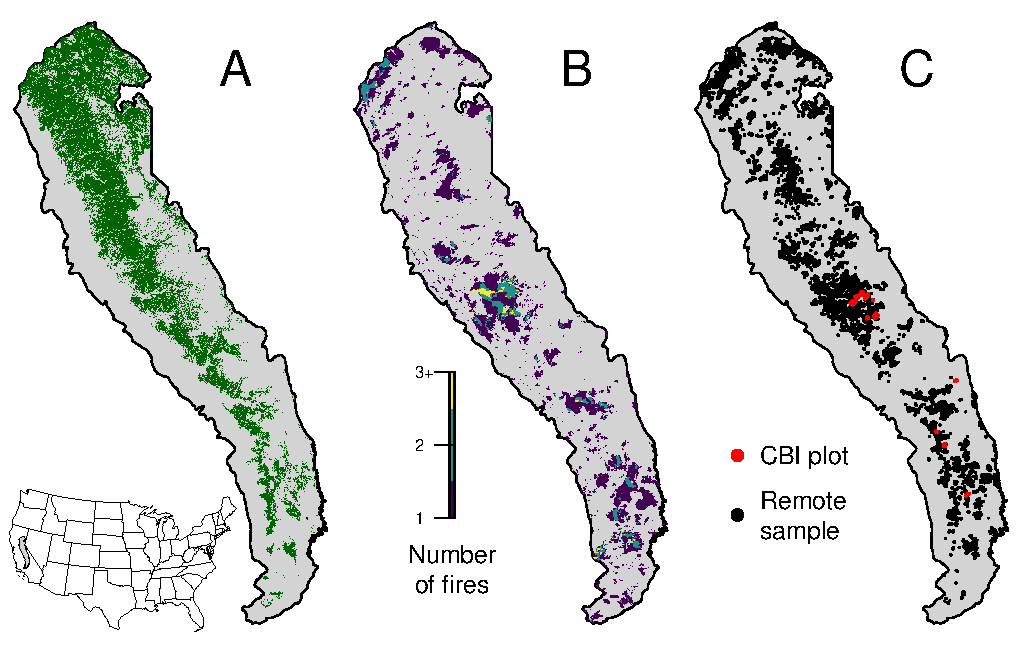
\includegraphics{../../figures/study-geographic-setting.pdf}
\caption{Fig. 1. Geographic setting of the study. A) Location of yellow
pine/mixed-conifer forests as designated by the Fire Return Interval
Departure (FRID) product which, among other things, describes the
potential vegetation in an area based on the pre-Euroamerican settlement
fire regime. B) Locations of all fires covering greater than 4 hectares
that burned in yellow pine/mixed-conifer forest between 1984 and 2018 in
the Sierra Nevada mountain range of California according to the State of
California Fire Resource and Assessment Program database, the most
comprehensive database of fire perimeters of its kind. Colors indicate
how many fire perimeters overlapped a given pixel within the study time
period. C) (red) Locations of 208 composite burn index (CBI) ground
plots used to calibrate the remotely sensed measures of severity.
(black) Locations of random samples drawn from 1008 unique fires
depicted in panel B that were in yellow pine/mixed-conifer forest as
depicted in panel A, and which were designated as ``burned'' by
exceeding a threshold relative burn ratio (RBR) determined by
calibrating the algorithm presented in this study with ground-based CBI
measurements.}
\end{figure}

Our study assesses the effect of vegetation structure on wildfire
severity in the Sierra Nevada mountain range of California in yellow
pine/mixed-conifer forests (Fig. 1; Supp. methods). This system is
dominated by a mixture of conifer species including ponderosa pine
(\emph{Pinus ponderosa} Lawson \& C. Lawson), sugar pine (\emph{Pinus
lambertiana} Douglas), incense-cedar (\emph{Calocedrus decurrens}
(Torr.) Florin), Douglas-fir (\emph{Pseudotsuga menziesii} (Mirb.)
Franco), white fir (\emph{Abies concolor} (Gord. \& Glend.) Lindl. ex
Hildebr.), and red fir (\emph{Abies magnifica} A. Murray bis),
angiosperm trees primarily including black oak (\emph{Quercus kelloggii}
Newberry), as well as shrubs (\emph{Ceanothus} spp.,
\emph{Arctostaphylos} spp.) (Safford \& Stevens 2017).

\hypertarget{programatically-assessing-wildfire-severity}{%
\subsection{Programatically assessing wildfire
severity}\label{programatically-assessing-wildfire-severity}}

We measured forest vegetation characteristics and wildfire severity
using imagery from the Landsat series of satellites post-processed to
surface reflectance using radiometric corrections (Masek \emph{et al.}
2006; Vermote \emph{et al.} 2016; USGS 2017b, a). Landsat satellites
image the entire Earth approximately every 16 days with a 30m pixel
resolution. We used Google Earth Engine for image collation and
processing (Gorelick \emph{et al.} 2017).

We calculated wildfire severity for the most comprehensive record of
fire perimeters in California: the Fire and Resource Assessment Program
(FRAP) fire perimeter database
(\url{https://frap.fire.ca.gov/frap-projects/fire-perimeters/}). The
FRAP database includes all known fires that covered more than 4
hectares, compared to the regional standard database which includes
fires covering greater than 80 hectares (Miller \& Safford 2012; Steel
\emph{et al.} 2018) and the national standard database Monitoring Trends
in Burn Severity (MTBS) which includes fires covering greater than 400
hectares in the western U.S. (Eidenshink \emph{et al.} 2007). Smaller
fire events are important contributors to fire regimes, but their
effects are often underrepresented in analyses of fire effects
(Randerson \emph{et al.} 2012). The FRAP perimeters are error-checked,
but it is possible that duplicated events are occasionally represented
in the database. Using the FRAP database, we quantified fire severity
within each perimeter of 1008 wildfires in the Sierra Nevada yellow
pine/mixed-conifer forest that burned between 1984 and 2018, which more
than doubles the number of fire events with severity assessments
compared to the regional standard database.

We created per-pixel median composites of collections of pre- and
postfire images for each fire to calculate common spectral indices of
wildfire severity. Prefire image collections spanned a fixed time window
ending the day before each fire's discovery date and postfire image
collections spanned the same fixed time window, exactly one year after
the prefire window. We tested four different time periods (16, 32, 48,
and 64 days) that defined the time window of the pre- and postfire image
collections, and seven common spectral indices of severity (RBR, dNBR,
RdNBR, dNBR2, RdNBR2, dNDVI, RdNDVI) for a total of 28 different means
to remotely measure wildfire severity (Supp. methods).

We calibrated these 28 severity metrics with 208 field assessments of
fire effects from previous studies (Zhu \emph{et al.} 2006; Sikkink
\emph{et al.} 2013). Severity was measured in the field as the overstory
component of the Composite Burn Index (CBI)-- a metric of vegetation
mortality across several vertical vegetation strata within a 30m
diameter field plot. The overstory component of CBI characterizes fire
effects to the overstory vegetation specifically, which includes both
dominant/co-dominant big trees as well as intermediate-sized subcanopy
trees (generally 10-25 cm DBH and 8-20m tall) (Key \& Benson 2006). CBI
ranges from 0 (no fire impacts) to 3 (very high fire impacts), and is a
common standard for calibrating remotely-sensed severity data in western
U.S. forests (Key \& Benson 2006; Miller \& Thode 2007; Miller \emph{et
al.} 2009; Cansler \& McKenzie 2012; Parks \emph{et al.} 2014, 2018;
Prichard \& Kennedy 2014). We extracted each spectral severity metric at
the CBI plot locations using both bilinear and bicubic interpolation
(Cansler \& McKenzie 2012; Parks \emph{et al.} 2014, 2018) and fit a
non-linear model:

\begin{enumerate}
\def\labelenumi{(\arabic{enumi})}
\tightlist
\item
  \(\label{eq-cbi-calibration} \text{remote\_severity} = \beta_0 + \beta_1 e^{\beta_2 \text{cbi\_overstory}}\)
\end{enumerate}

We treated the spectral severity measure as the dependent variable in
this nonlinear regression for comparison with other studies (Miller \&
Thode 2007; Miller \emph{et al.} 2009; Parks \emph{et al.} 2014). We
performed ten-fold cross validation using the \texttt{modelr} and
\texttt{purrr} packages (Henry \& Wickham 2019; Wickham 2019) and report
the average R\textsuperscript{2} value for each model. We used the
severity calculation derived from the best fitting model for all further
analyses (Relative Burn Ratio {[}RBR{]} calculated using a 48-day time
window; ten-fold cross validation \(R^2 =\) 0.806; first panel of Fig.
2; Supp. Table 1).

\begin{figure}
\centering
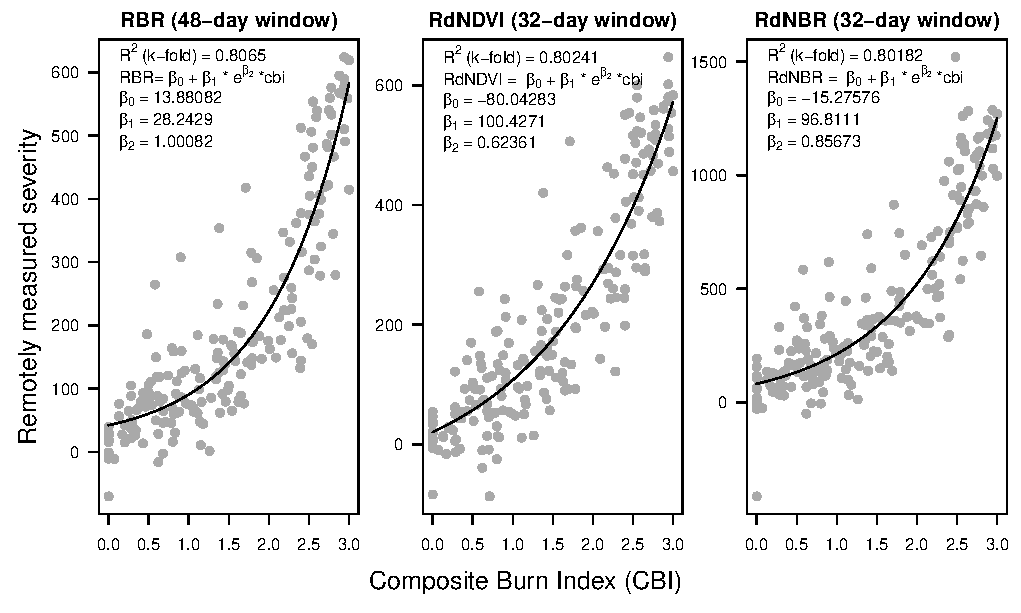
\includegraphics{../../figures/remote-sensed-severity-calibration.pdf}
\caption{Fig. 2. Three top performing remotely-sensed severity metrics
based on ten-fold cross validation (relative burn ratio, 48-day window,
bicubic interpolation; relative delta normalized burn ratio, 32-day
window, bilinear interpolation; and relative delta normalized difference
vegetation index, 48-day window, bilinear interpolation) calculated
using new automated image collation algorithms, calibrated to 208 field
measures of fire severity (composite burn index). See Supplemental Table
1 for performance of all tested models.}
\end{figure}

\begin{figure}
\centering
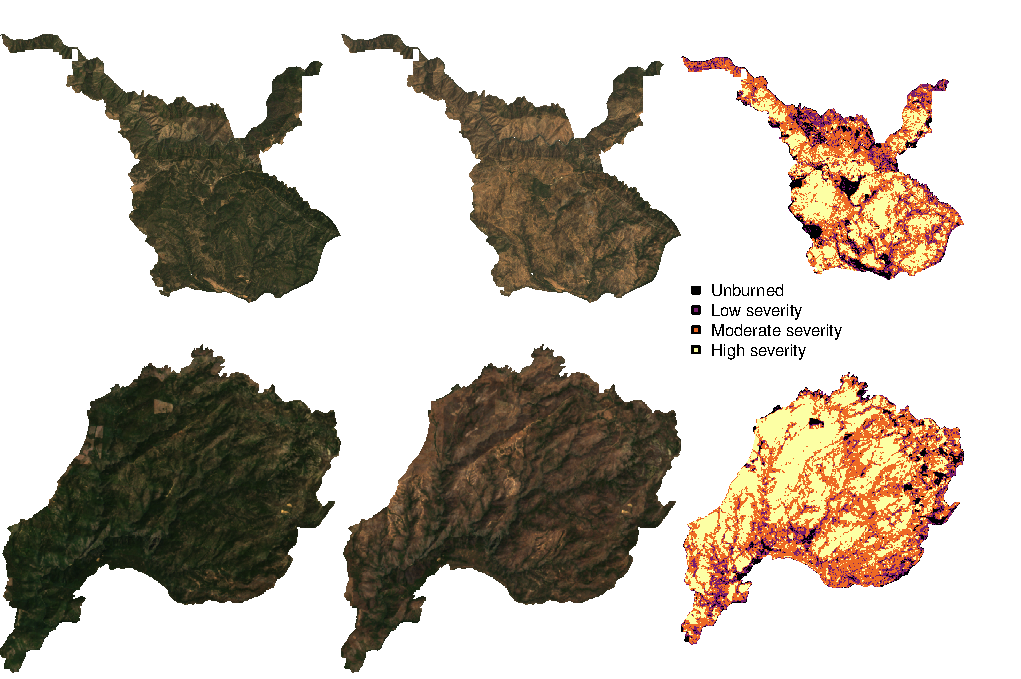
\includegraphics{../../figures/pre-post-rbr.pdf}
\caption{Fig. 3. Example algorithm outputs for the Hamm Fire of 1987
(top half) and the American Fire of 2013 (bottom half) showing: prefire
true color composite image (left third), postfire true color composite
image (center third), relative burn ratio (RBR) calculation using a
48-day image collation window before the fire and one year later (right
third). For visualization purposes, the continous severity index has
been binned into severity categories.}
\end{figure}

Using the non-linear relationship between RBR and CBI, we calculated the
threshold RBR corresponding to ``high-severity'' signifying complete or
near-complete overstory mortality using the common CBI high-severity
lower threshold of 2.25 (i.e., an RBR value of 282.335; Fig. 3) (Miller
\& Thode 2007).

\hypertarget{assessing-local-forest-structure-variability-at-broad-extents}{%
\subsection{Assessing local forest structure variability at broad
extents}\label{assessing-local-forest-structure-variability-at-broad-extents}}

We used texture analysis to calculate a remotely-sensed measure of local
forest variability (Haralick \emph{et al.} 1973; Tuanmu \& Jetz 2015).
Within a moving square neighborhood window with sides of 90m (3x3
pixels), 150m (5x5 pixels), 210m (7x7 pixels), and 270m (9x9 pixels), we
calculated forest variability for each pixel as the standard deviation
of the NDVI values of its neighbors (not including itself). NDVI
correlates well with foliar biomass, leaf area index, and vegetation
cover (Rouse \emph{et al.} 1973), so a higher standard deviation of NDVI
within a given local neighborhood corresponds to discontinuous canopy
cover and abrupt vegetation edges (see Fig. 4) (Franklin \emph{et al.}
1986).

\begin{figure}
\centering
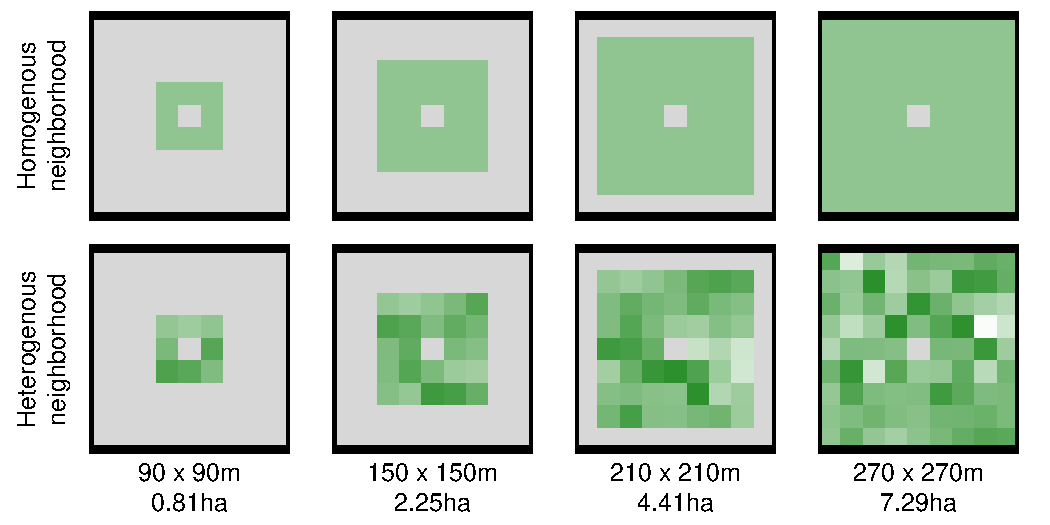
\includegraphics{../../figures/heterogeneity-demo-raster.pdf}
\caption{Fig. 4. Example of homogenous forest (top row) and heterogenous
forest (bottom row) with the same mean NDVI values
(\textasciitilde{}0.6). Each column represents forest structural
variability measured using a different neighborhood size. NDVI is
represented by a white to green color gradient, and pixels that are not
included in the forest structural variability metric are colored gray.}
\end{figure}

\hypertarget{assessing-other-conditions}{%
\subsection{Assessing other
conditions}\label{assessing-other-conditions}}

Elevation data were sourced from a 1-arc second digital elevation model
(DEM) (Farr \emph{et al.} 2007) which was used to calculate slope,
aspect, and potential annual heat load-- an integrated measure of
latitude, slope, and aspect (McCune \& Keon (2002); Supp. methods).
Per-pixel topographic roughness was calculated as the standard deviation
of elevation values within the same-sized kernels as those used for
variability in forest structure (90m, 150m, 210m, and 270m on a side and
not including the central pixel). We chose this specific measure of
topographic roughness because it directly parallels and accounts for our
metric of forest structure variability and because of its use in other
studies (Holden \emph{et al.} 2009), though other measures of
topographic heterogeneity have been used for fire modeling (Haire \&
McGarigal 2009; Holden \emph{et al.} 2009; Cansler \& McKenzie 2014).

We calculated prefire fuel moisture as the median 100-hour fuel moisture
for the 3 days prior to the fire using gridMET, a gridded meteorological
product with a daily temporal resolution and a 4km x 4km spatial
resolution (Abatzoglou 2013). The 100-hour fuel moisture is a correlate
of the regional temperature and moisture which integrates the relative
humidity, the length of day, and the amount of precipitation in the
previous 24 hours. Thus, this measure is sensitive to multiple hot dry
days across the 4km x 4km spatial extent of each grid cell, but not to
diurnal variation in relative humidity nor to extreme weather events
during a fire.

\hypertarget{modeling}{%
\subsection{Modeling}\label{modeling}}

Approximately 100 random points were selected within each FRAP fire
perimeter in areas designated as yellow pine/mixed-conifer forest and we
extracted the values of severity and covariate at those points using
nearest neighbor interpolation. Using the calibration equation described
in Eq. 1 for the best configuration of the remote severity metric, we
removed sampled points corresponding to ``unburned'' area prior to
analysis (i.e., below an RBR threshold of 45.097). The random sampling
amounted to 56088 total samples across 1008 fires.

We used a hierarchical logistic regression model (Eq. 2) to assess the
probability of high-severity wildfire as a linear combination of the
remote metrics described above: prefire NDVI of each pixel, standard
deviation of NDVI within a neighborhood (i.e., forest structural
variability), the mean NDVI within a neighborhood, 100-hour fuel
moisture, potential annual heat load, and topographic roughness. We
included two-way interactions between the structural variability measure
and prefire NDVI, neighborhood mean NDVI, and 100-hour fuel moisture. We
include the two-way interaction between a pixel's prefire NDVI and its
neighborhood mean NDVI to account for structural variability that may
arise from contrasts between these variables (e.g., ``holes in the
forest'' vs. ``isolated patches''; Supp. Fig. 2). We scaled all
predictor variables, used weakly-regularizing priors, and estimated an
intercept for each individual fire with pooled variance (i.e., a
group-level effect of fire). We used the \texttt{brms} package to fit
models in a Bayesian framework which implements the No U-Turn Sampler
extension to the Hamiltonian Monte Carlo algorithm (Hoffman \& Gelman
2014; Bürkner 2017). We used 4 chains with 5000 samples per chain
(including 2500 warmup samples) and chain convergence was assessed for
each estimated parameter by ensuring Rhat values were less than or equal
to 1.01 (Bürkner 2017).

\begin{enumerate}
\def\labelenumi{(\arabic{enumi})}
\setcounter{enumi}{1}
\tightlist
\item
  \(\begin{aligned} \label{eq-severity-model} severity_{i, j} &\sim Bern(\phi_{i,j}) \\ logit(\phi_{i,j}) &= \begin{aligned} & \beta_0 + \\ & \beta_{\text{nbhd\_stdev\_NDVI}} * \text{nbhd\_stdev\_NDVI}_i + \\ & \beta_{\text{prefire\_NDVI}} * \text{prefire\_NDVI}_i + \\ & \beta_{\text{nbhd\_mean\_NDVI}} * \text{nbhd\_mean\_NDVI}_i + \\ & \beta_{\text{fm100}} * \text{fm100}_i + \\ & \beta_{\text{pahl}} * \text{pahl}_i + \\ & \beta_{\text{topographic\_roughness}} * \text{topographic\_roughness}_i + \\ & \beta_{\text{nbhd\_stdev\_NDVI*fm100}} * \text{nbhd\_stdev\_NDVI}_i * \text{fm100}_i + \\ & \beta_{\text{nbhd\_stdev\_NDVI*prefire\_NDVI}} * \text{nbhd\_stdev\_NDVI}_i * \text{prefire\_NDVI}_i + \\ & \beta_{\text{nbhd\_stdev\_NDVI*nbhd\_mean\_NDVI}} * \text{nbhd\_stdev\_NDVI}_i * \text{nbhd\_mean\_NDVI}_i + \\ & \beta_{\text{nbhd\_mean\_NDVI*prefire\_NDVI}} * \text{nbhd\_mean\_NDVI}_i * \text{prefire\_NDVI}_i + \\ & \gamma_j \end{aligned} \\ \gamma_j &\sim \mathcal{N}(0, \sigma_{\text{fire}}) \end{aligned}\)
\end{enumerate}

\hypertarget{scale-of-effect-of-forest-structure-variability}{%
\subsection{Scale of effect of forest structure
variability}\label{scale-of-effect-of-forest-structure-variability}}

Each neighborhood size (90m, 150m, 210m, 270m) was substituted in turn
for the neighborhood standard deviation of NDVI, neighborhood mean NDVI,
and terrain roughness covariates to generate a candidate set of 4
models. To assess the scale at which these neighborhood-size-dependent
effects manifested, we compared the 4 candidate models using
leave-one-out cross validation (Vehtari \emph{et al.} 2017). We inferred
that the neighborhood size window used in the best-performing model
reflected the scale at which the forest structure variability effect had
the most support (Graham \emph{et al.} 2019). We used \texttt{R} for all
statistical analyses (R Core Team 2018).

\hypertarget{results}{%
\section{Results}\label{results}}

Our programmatic assessment of wildfire severity calibrates as well or
better than other reported methods that often require substantial manual
intervention (Edwards \emph{et al.} 2018). We found that this approach
was robust to a wide range of spectral severity metrics, time windows,
and interpolation techniques, including those based on NDVI are
seldom-used in this system (Fig. 2; Supp. Tab. 1; Supp. methods).

\begin{longtable}[]{@{}ccccccc@{}}
\caption{Tab. 1: Comparison of four models described in Eq.
\ref{eq-severity-model} using different neighborhood sizes for
calculating forest structural variability (standard deviation of NDVI
within the neighborhood), neighborhood mean NDVI, and topographic
roughness (standard deviation of elevation within the neighborhood). LOO
is a measure of a model's predictive accuracy (with lower values
corresponding to more accurate prediction) and is calculated as -2 times
the expected log pointwise predictive density (elpd) for a new dataset
(Vehtari \emph{et al.} 2017). \(\Delta\)LOO is the difference between a
model's LOO and the lowest LOO in a set of models (i.e., the model with
the best predictive accuracy). The Bayesian \(R^2\) is a `data-based
estimate of the proportion of variance explained for new data' (Gelman
\emph{et al.} 2018). Note that Bayesian \(R^2\) values are conditional
on the model so shouldn't be compared across models, though they can be
informative about a single model at a time.}\tabularnewline
\toprule
\begin{minipage}[b]{0.06\columnwidth}\centering
Model\strut
\end{minipage} & \begin{minipage}[b]{0.17\columnwidth}\centering
Neighborhood size for variability measure\strut
\end{minipage} & \begin{minipage}[b]{0.09\columnwidth}\centering
LOO (-2*elpd)\strut
\end{minipage} & \begin{minipage}[b]{0.11\columnwidth}\centering
\(\Delta\) LOO to best model\strut
\end{minipage} & \begin{minipage}[b]{0.11\columnwidth}\centering
SE of \(\Delta\) LOO\strut
\end{minipage} & \begin{minipage}[b]{0.16\columnwidth}\centering
LOO model weight (\%)\strut
\end{minipage} & \begin{minipage}[b]{0.11\columnwidth}\centering
Bayesian R\textsuperscript{2}\strut
\end{minipage}\tabularnewline
\midrule
\endfirsthead
\toprule
\begin{minipage}[b]{0.06\columnwidth}\centering
Model\strut
\end{minipage} & \begin{minipage}[b]{0.17\columnwidth}\centering
Neighborhood size for variability measure\strut
\end{minipage} & \begin{minipage}[b]{0.09\columnwidth}\centering
LOO (-2*elpd)\strut
\end{minipage} & \begin{minipage}[b]{0.11\columnwidth}\centering
\(\Delta\) LOO to best model\strut
\end{minipage} & \begin{minipage}[b]{0.11\columnwidth}\centering
SE of \(\Delta\) LOO\strut
\end{minipage} & \begin{minipage}[b]{0.16\columnwidth}\centering
LOO model weight (\%)\strut
\end{minipage} & \begin{minipage}[b]{0.11\columnwidth}\centering
Bayesian R\textsuperscript{2}\strut
\end{minipage}\tabularnewline
\midrule
\endhead
\begin{minipage}[t]{0.06\columnwidth}\centering
1\strut
\end{minipage} & \begin{minipage}[t]{0.17\columnwidth}\centering
90 x 90m\strut
\end{minipage} & \begin{minipage}[t]{0.09\columnwidth}\centering
42364\strut
\end{minipage} & \begin{minipage}[t]{0.11\columnwidth}\centering
0\strut
\end{minipage} & \begin{minipage}[t]{0.11\columnwidth}\centering
NA\strut
\end{minipage} & \begin{minipage}[t]{0.16\columnwidth}\centering
100\strut
\end{minipage} & \begin{minipage}[t]{0.11\columnwidth}\centering
0.300\strut
\end{minipage}\tabularnewline
\begin{minipage}[t]{0.06\columnwidth}\centering
2\strut
\end{minipage} & \begin{minipage}[t]{0.17\columnwidth}\centering
150 x 150m\strut
\end{minipage} & \begin{minipage}[t]{0.09\columnwidth}\centering
42417\strut
\end{minipage} & \begin{minipage}[t]{0.11\columnwidth}\centering
53.17\strut
\end{minipage} & \begin{minipage}[t]{0.11\columnwidth}\centering
14.99\strut
\end{minipage} & \begin{minipage}[t]{0.16\columnwidth}\centering
0\strut
\end{minipage} & \begin{minipage}[t]{0.11\columnwidth}\centering
0.299\strut
\end{minipage}\tabularnewline
\begin{minipage}[t]{0.06\columnwidth}\centering
3\strut
\end{minipage} & \begin{minipage}[t]{0.17\columnwidth}\centering
210 x 210m\strut
\end{minipage} & \begin{minipage}[t]{0.09\columnwidth}\centering
42459\strut
\end{minipage} & \begin{minipage}[t]{0.11\columnwidth}\centering
94.44\strut
\end{minipage} & \begin{minipage}[t]{0.11\columnwidth}\centering
21.35\strut
\end{minipage} & \begin{minipage}[t]{0.16\columnwidth}\centering
0\strut
\end{minipage} & \begin{minipage}[t]{0.11\columnwidth}\centering
0.299\strut
\end{minipage}\tabularnewline
\begin{minipage}[t]{0.06\columnwidth}\centering
4\strut
\end{minipage} & \begin{minipage}[t]{0.17\columnwidth}\centering
270 x 270m\strut
\end{minipage} & \begin{minipage}[t]{0.09\columnwidth}\centering
42491\strut
\end{minipage} & \begin{minipage}[t]{0.11\columnwidth}\centering
126.5\strut
\end{minipage} & \begin{minipage}[t]{0.11\columnwidth}\centering
25.15\strut
\end{minipage} & \begin{minipage}[t]{0.16\columnwidth}\centering
0\strut
\end{minipage} & \begin{minipage}[t]{0.11\columnwidth}\centering
0.298\strut
\end{minipage}\tabularnewline
\bottomrule
\end{longtable}

The model with the best out-of-sample prediction accuracy assessed by
leave-one-out cross validation was the model fit using the smallest
neighborhood size for the variability of forest structure (standard
deviation of neighborhood NDVI), the mean of neighborhood NDVI, and the
terrain roughness (standard deviation of elevation) (Tab. 1). One
hundred percent of the model weight belongs to the model using the
smallest neighborhood size window.

\begin{figure}
\centering
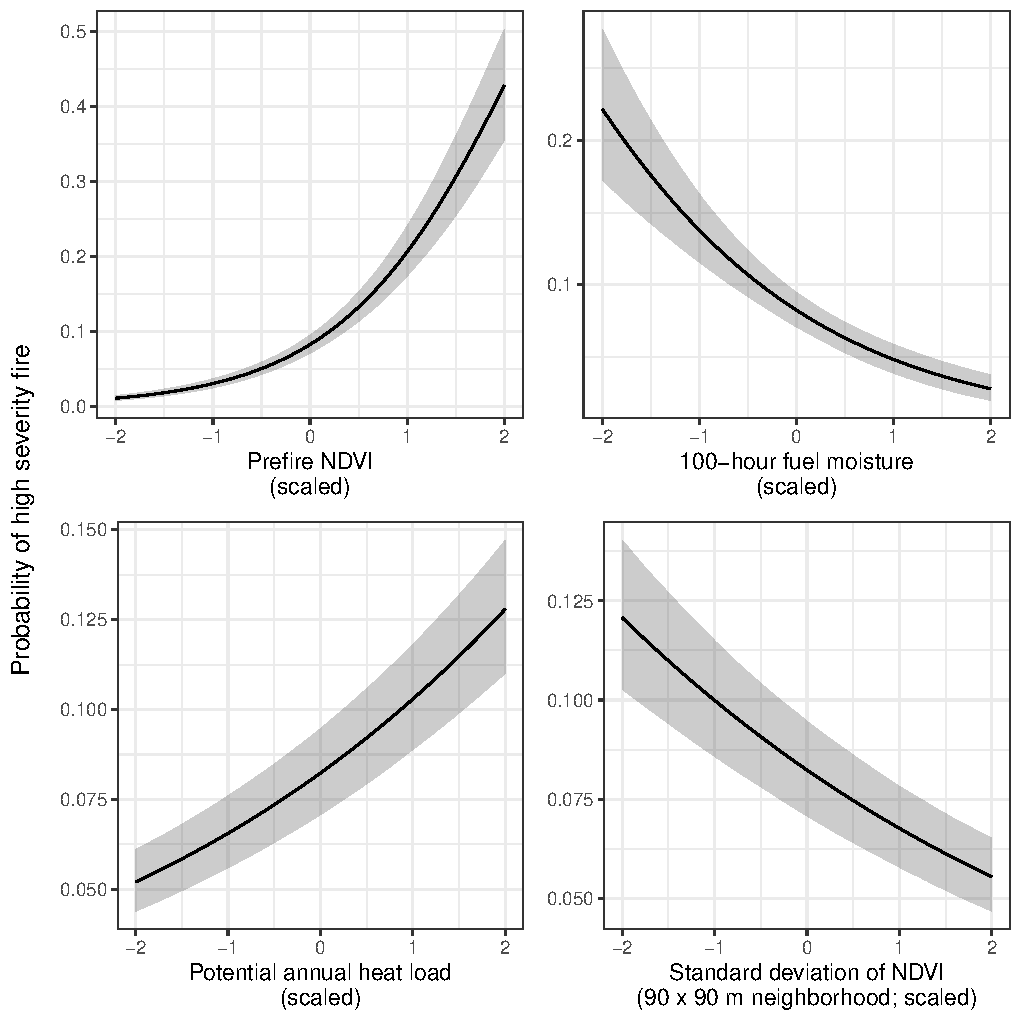
\includegraphics{../../figures/prob-hi-sev-main-effects-credible-intervals.pdf}
\caption{Fig. 5. The main effects and 95\% credible intervals of the
covariates having the strongest relationships with the probability of
high-severity fire. All depicted relationships derive from the model
using the 90m x 90m neighborhood size window for neighborhood standard
deviation of NDVI, neighborhood mean of NDVI, and topographic roughness,
as this was the best performing model of the four neighborhood sizes
tested. The effect sizes of these covariates were similar for each
neighborhood size tested.}
\end{figure}

We report the results from fitting the model described in Eq. 2 using
the smallest neighborhood size (90 x 90m) because this was the best
performing model (see above) and because the size and magnitude of
estimated coefficients were similar across neighborhood sizes (Supp.
Tab. 2).

The strongest influence on the probability of a forested area burning at
high-severity was the a pixel's prefire NDVI, with a greater prefire
NDVI increasing the probability of high-severity fire
(\(\beta_{\text{prefire\_ndvi}}=\) 1.06; 95\% CI: {[}0.931, 1.192{]});
Fig. 5). There was a strong negative relationship between 100-hour fuel
moisture and wildfire severity such that increasing 100-hour fuel
moisture was associated with a decreasing probability of a high-severity
wildfire (\(\beta_{\text{fm100}}=\) -0.576; 95\% CI: {[}-0.709,
-0.442{]}) (Fig. 5). Potential annual heat load, which integrates
aspect, slope, and latitude, also had a strong positive relationship
with the probability of a high-severity fire. Areas that were located on
southwest facing sloped terrain at lower latitudes had the highest
potential annual heat load, and were more likely to burn at
high-severity (\(\beta_{\text{pahl}}=\) 0.246; 95\% CI: {[}0.215,
0.277{]}) Fig. 5). We found a negative effect of the prefire
neighborhood mean NDVI on the probability of a pixel burning at
high-severity (\(\beta_{\text{nbhd\_mean\_NDVI}}=\) -0.168; 95\% CI:
{[}-0.311, -0.028{]}). This is in contrast to the positive effect of the
prefire NDVI of the pixel itself. We found no effect of local
topographic roughness on wildfire severity
(\(\beta_{\text{topographic\_roughness}}=\) 0.002; 95\% CI: {[}-0.029,
0.034{]}).

There was also a strong negative interaction between the neighborhood
mean NDVI and the prefire NDVI of the central pixel
(\(\beta_{\text{nbhd\_mean\_NDVI*prefire\_NDVI}}\) -0.54; 95\% CI:
{[}-0.587, -0.494{]}).

From the same model, we found strong evidence for a negative effect of
variability of vegetation structure on the probability of a
high-severity wildfire (\(\beta_{\text{nbhd\_stdev\_NDVI}}=\) -0.213;
95\% CI: {[}-0.251, -0.174{]}); Fig. 5). We also found significant
interactions between variability of vegetation structure and prefire
NDVI of the central pixel
\(\beta_{\text{nbhd\_stdev\_NDVI*prefire\_NDVI}}=\) 0.128; 95\% CI:
{[}0.031, 0.221{]}) as well as between variability of vegetation
structure and neighborhood mean NDVI
(\(\beta_{\text{nbhd\_stdev\_NDVI*nbhd\_mean\_NDVI}}=\) -0.115; 95\% CI:
{[}-0.206, -0.022{]}).

\hypertarget{discussion}{%
\section{Discussion}\label{discussion}}

Broad-extent, fine-grain, spatially-explicit analyses of whole
ecosystems are key to illuminating macroecological phenomena such as
forest resilience to disturbance (Heffernan \emph{et al.} 2014). We used
a powerful, cloud-based geographic information system and data
repository, Google Earth Engine, as a `macroscope' (Beck \emph{et al.}
2012) to study feedbacks between vegetation structure and wildfire
disturbance in yellow pine/mixed-conifer forests of California's Sierra
Nevada mountain range. With this approach, we reveal and quantify
general features of this forest system, and gain deeper insights into
the mechanisms underlying its function.

\hypertarget{high-severity-wildfire-and-ecological-resilience}{%
\subsection{High-severity wildfire and ecological
resilience}\label{high-severity-wildfire-and-ecological-resilience}}

Wildfire severity can be considered a direct correlate of a forest's
resistance-- the ease or difficulty with which a disturbance changes the
system state (Folke \emph{et al.} 2004; Walker \emph{et al.} 2004). One
relevant state change for assessing ecosystem resistance is the loss of
its characteristic native biota (Keith \emph{et al.} 2013), which could
be represented as overstory tree mortality (e.g., severity) in a
forested system. The same fire behavior in two different forest systems
(e.g., old-growth conifer versus young conifer plantation) may have very
different abilities to cause overstory mortality (Keeley 2009), which
reflects differences in each forest's resistance. Resistance is a key
component of resilience (Folke \emph{et al.} 2004; Walker \emph{et al.}
2004) and, in this framework, one manifestation of forest resilience is
high resistance to wildfire, whereby some mechanism leads to lower
severity when a fire occurs. Here, we show clear evidence that
structural heterogeneity fulfills this mechanistic resistance role in
dry coniferous systems (Fig. 5). This study thus provides a particularly
extensive, large-scale example of an association between local
structural heterogeneity and ecosystem resilience, a phenomenon that has
been demonstrated in other systems at smaller scales.

These findings do not imply that resistance to fire is a sole or
necessary path to resilience. For instance, high-severity fire is
characteristic of other forest systems such as serotinous lodgepole pine
forests in Yellowstone National Park, and is not ordinarily expected to
hamper forest regeneration (Turner \emph{et al.} 1997). Our inference
that structural variability is a fundamental resilience mechanism in dry
coniferous forests is strengthened by its large effect size and our
ability to measure the negative feedback phenomenon at relevant
spatiotemporal scales: we captured local-scale variability in structure
and wildfire severity at broad spatial extents for an extensive set of
over 1,000 fires across a 34-year time span.

\hypertarget{factors-influencing-the-probability-of-high-severity-wildfire}{%
\subsection{Factors influencing the probability of high-severity
wildfire}\label{factors-influencing-the-probability-of-high-severity-wildfire}}

We found that the strongest influence on the probability of
high-severity wildfire was prefire NDVI. Greater NDVI corresponds to
high canopy cover and vegetation density (Rouse \emph{et al.} 1973)
which translates directly to live fuel loads in the forest canopy and
can increase high-severity fire (Parks \emph{et al.} 2018). Overstory
canopy cover and density also correlate (though weakly) with surface
fuel loads (Lydersen \emph{et al.} 2015; Collins \emph{et al.} 2016;
Cansler \emph{et al.} 2019), which can play a large role in driving
high-severity fire in these forests (Agee 1996). Thus NDVI is likely a
strong predictor of fire severity because it is correlated with both
surface fuel loads and canopy live fuel density.

We found a strong positive effect of potential annual heat load as well
as a strong negative effect of 100-hour fuel moisture, results which
corroborates similar studies (Parks \emph{et al.} 2018). Some work has
shown that terrain roughness (Haire \& McGarigal 2009; Holden \emph{et
al.} 2009; Dillon \emph{et al.} 2011; Krawchuk \emph{et al.} 2016) can
be an important predictor of wildfire severity, but we found no effect
using our measure of local terrain variability. This may be a function
of scale-- our measures of topographic roughness were more localized
than those of other studies (Holden \emph{et al.} 2009; Dillon \emph{et
al.} 2011). Haire \& McGarigal (2009) also found occasional instances
where small differences in topographic roughness had dramatic
differences in severity. These sorts of influences on severity would be
challenging to detect in our modeling framework, which was designed to
estimate an overall influence of topographic roughness on fire severity.
Also, topographic roughness could be measured in different ways that
highlight different types of heterogeneity (Haralick \emph{et al.}
1973), which suggests that an effect of topographic roughness on mean
wildfire severity will be best-captured by a roughness measure that
aligns with the dominant phenomenon driving that effect. Finally, the
observed influence of topographic roughness in other studies may have
been fully or partially driven by variability in vegetation, which we
partition separately in our study.

Critically, we found a strong negative effect of forest structural
variability on wildfire severity that was opposite in direction but
similar in magnitude to the effect of potential annual heat load. Just
as the positive effect of NDVI is likely driven by increased fuel loads,
the negative effect of variability in NDVI, is likely driven by
discontinuity in surface, ladder, and canopy fuels, which can reduce the
probability of initiation and spread of tree-killing crown fires (Wagner
1977; Agee 1996; Graham \emph{et al.} 2004). This discontinuity can
manifest in a number of ways. For instance, neighboring forest pixels
with different tree size distributions may disrupt a crown fire's spread
from a low to a high crown or vice versa. Local NDVI variability may
also reflect heterogeneous arrangement of vegetation types such as a
forested pixel adjacent to a pixel mostly covered by grass. In the
grass-dominated area, the relatively low flame heights would likely fail
to initiate or sustain active crowning behavior that would kill
overstory trees in the neighboring forested area. Finally, forest
structural variability may also arise with different land cover types in
the local neighborhood that influence severity, such as when exposed
bedrock or a group of boulders acts as fire refugia for vegetation
rooted within it (Hylander \& Johnson 2010).

\hypertarget{feedback-between-forest-structural-variability-and-wildfire-severity}{%
\subsection{Feedback between forest structural variability and wildfire
severity}\label{feedback-between-forest-structural-variability-and-wildfire-severity}}

This system-wide inverse relationship between structural variability and
wildfire severity closes a feedback that links past and future fire
behavior via forest structure. Frequent wildfire in dry coniferous
forests generates variable forest structure (North \emph{et al.} 2009;
Larson \& Churchill 2012; Malone \emph{et al.} 2018), which in turn, as
we demonstrate, dampens the severity of future fire. In contrast,
exclusion of wildfire homogenizes forest structure and increases the
probability that a fire will produce large, contiguous patches of
overstory mortality (Stevens \emph{et al.} 2017; Steel \emph{et al.}
2018). The proportion and spatial configuration of fire severity in
fire-prone forests are key determinants of their long-term persistence
(Stevens \emph{et al.} 2017; Steel \emph{et al.} 2018). Lower-severity
fire or scattered patches of higher-severity fire reduce the risk of
conversion to a non-forest vegetation type (Kemp \emph{et al.} 2016;
Stevens-Rumann \emph{et al.} 2018; Walker \emph{et al.} 2018), while
prospects for forest regeneration are bleaker when high-severity patch
sizes are much larger than the natural range of variation for the system
(Miller \& Safford 2017; Stevens \emph{et al.} 2017; Stevens-Rumann \&
Morgan 2019). Thus, the forest-structure-mediated feedback between past
and future fire severity underlies the resilience of the Sierra Nevada
yellow pine/mixed-conifer system.

\hypertarget{scale-of-effect-of-variability-in-forest-structure}{%
\subsection{Scale of effect of variability in forest
structure}\label{scale-of-effect-of-variability-in-forest-structure}}

We found that the effect of a forest patch's neighborhood
characteristics on the probability of high-severity fire was strongest
at the smallest neighborhood size that we tested, 90 x 90m. This
suggests that the moderating effect of forest structure variability on
fire severity is a very local phenomenon. This corroborates work by
Safford \emph{et al.} (2012), who found that crown fires (high
tree-killing potential) were almost always reduced to surface fires (low
tree-killing potential) within 70m of entering a fuel reduction
treatment area.

Severity patterns at a landscape scale (e.g., for a whole fire) may
represent cross-scale emergences of the local influence of forest
structure variability on fire effects (Peters \emph{et al.} 2004; Rose
\emph{et al.} 2017). For instance, forest management actions (e.g.,
prescribed fire, use of wildfire under mild conditions) that reduce fuel
loads and increase structural variability can be effective at reducing
fire severity across broader spatial extents than the direct footprints
of those actions (Graham \emph{et al.} 2004; Stephens \emph{et al.}
2009; Tubbesing \emph{et al.} 2019). Some work suggests that this sort
of cross-scale emergence may depend on even broader-scale effects of
fire weather, with small-scale variability failing to influence fire
behavior under extreme conditions (Peters \emph{et al.} 2004; Lydersen
\emph{et al.} 2014), though we did not detect such an interaction
between our metric of burning conditions (100-hour fuel moisture) and
forest structure variability.

\hypertarget{correlation-between-covariates-and-interactions}{%
\subsection{Correlation between covariates and
interactions}\label{correlation-between-covariates-and-interactions}}

Unexpectedly, we found a strong interaction between the prefire NDVI at
a pixel and its neighborhood mean NDVI on the probability of
high-severity fire. These two variables are strongly correlated
(\(\text{Spearman's }\rho=\) 0.97), so the general effect of this
interaction is to dampen the dominating effect of prefire NDVI. Thus,
though the marginal effect of prefire NDVI on the probability of
high-severity fire is still positive and large, its real-world effect
might be more comparable to other modeled covariates when including the
negative main effect of neighborhood mean NDVI, the negative interaction
effect of prefire NDVI and neighborhood mean NDVI, and their tendency to
covary (compare the effect of prefire NDVI under the common scenario of
prefire NDVI and neighborhood mean NDVI increasing or decreasing
together:
\(\beta_{\text{prefire\_ndvi}}+\beta_{\text{nbhd\_mean\_NDVI}}+\beta_{\text{nbhd\_mean\_NDVI*prefire\_NDVI}}=\)
0.352, to the effect of 100-hour fuel moisture, which becomes the effect
with the greatest magnitude: \(\beta_{\text{fm100}}=\) -0.576).

In the few cases when prefire NDVI and the neighborhood mean NDVI
contrast, there is an overall effect of increasing the probability of
high-severity fire. When prefire NDVI at the central pixel is high and
the neighborhood NDVI is low (e.g., an isolated vegetation patch;
Supplemental Fig. 2), the probability of high-severity fire is expected
to dramatically increase. When prefire NDVI at the central pixel is low
and the neighborhood NDVI is high (e.g., a hole in the forest; Supp.
Fig. 2), the probability of high-severity fire at that central pixel is
still expected to be fairly high even though vegetation is sparse there.
In these forest NDVI datasets, when these variables do decouple, they
tend to do so in the ``hole in the forest'' case and lead to a greater
probability of high-severity fire at the central pixel despite its low
NDVI. This can perhaps be explained if the consistently high vegetation
density in a local neighborhood-- itself more likely to burn at
high-severity-- exerts a contagious effect on the central pixel, raising
its probability of burning at high-severity regardless of how much fuel
might be there to burn.

\hypertarget{conclusions}{%
\subsection{Conclusions}\label{conclusions}}

Theory and empirical work suggest a general link between forest
structural heterogeneity and resilience. Here we find strong evidence
with a large-scale study that, across large areas of forest, variable
forest structure generally makes yellow pine/mixed-conifer forest in the
Sierra Nevada more resistant to inevitable wildfire disturbance. It has
been well-documented that frequent, low-severity wildfire maintains
forest structural variability. Here, we demonstrate a system-wide
reciprocal effect suggesting that greater local-scale variability of
vegetation structure makes fire-prone, dry forests more resilient to
wildfire and may increase the probability of their long-term
persistence.

\hypertarget{acknowledgements}{%
\section{Acknowledgements}\label{acknowledgements}}

We thank Connie Millar, Derek Young, and Meagan Oldfather for valuable
comments about this work and we also thank the community of Google Earth
Engine developers for prompt and helpful insights about the platform. We
thank four anonymous reviewers for their helpful comments on the
manuscript. Funding for this work was provided by NSF Graduate Research
Fellowship Grant \#DGE- 1321845 Amend. 3 as well as by Earth Lab through
CU Boulder's Grand Challenge Initiative and the Cooperative Institute
for Research in Environmental Sciences (CIRES) at CU Boulder (to MJK).

\hypertarget{references}{%
\section*{References}\label{references}}
\addcontentsline{toc}{section}{References}

\hypertarget{refs}{}
\leavevmode\hypertarget{ref-abatzoglou2013}{}%
1.\\
Abatzoglou, J.T. (2013). Development of gridded surface meteorological
data for ecological applications and modelling. \emph{International
Journal of Climatology}, 33, 121--131.

\leavevmode\hypertarget{ref-abatzoglou2016}{}%
2.\\
Abatzoglou, J.T. \& Williams, A.P. (2016). Impact of anthropogenic
climate change on wildfire across western U.S. Forests.
\emph{Proceedings of the National Academy of Sciences}, 113,
11770--11775.

\leavevmode\hypertarget{ref-agee1996}{}%
3.\\
Agee, J.K. (1996). The influence of forest structure on fire behavior.
\emph{17th Forest Vegetation Management Conference}, 17.

\leavevmode\hypertarget{ref-beck2012}{}%
4.\\
Beck, J., Ballesteros-Mejia, L., Buchmann, C.M., Dengler, J., Fritz,
S.A. \& Gruber, B. \emph{et al.} (2012). What's on the horizon for
macroecology? \emph{Ecography}, 35, 673--683.

\leavevmode\hypertarget{ref-bessie1995}{}%
5.\\
Bessie, W.C. \& Johnson, E.A. (1995). The relative importance of fuels
and weather on fire behavior in subalpine forests. \emph{Ecology}, 76,
747--762.

\leavevmode\hypertarget{ref-burkner2017}{}%
6.\\
Bürkner, P.-C. (2017). \textbf{brms}: An \emph{R} package for bayesian
multilevel models using \emph{Stan}. \emph{Journal of Statistical
Software}, 80.

\leavevmode\hypertarget{ref-cansler2012}{}%
7.\\
Cansler, C.A. \& McKenzie, D. (2012). How robust are burn severity
indices when applied in a new region? Evaluation of alternate
field-based and remote-sensing methods. \emph{Remote Sensing}, 4,
456--483.

\leavevmode\hypertarget{ref-cansler2014}{}%
8.\\
Cansler, C.A. \& McKenzie, D. (2014). Climate, fire size, and
biophysical setting control fire severity and spatial pattern in the
northern Cascade Range, USA. \emph{Ecological Applications}, 24,
1037--1056.

\leavevmode\hypertarget{ref-cansler2019}{}%
9.\\
Cansler, C.A., Swanson, M.E., Furniss, T.J., Larson, A.J. \& Lutz, J.A.
(2019). Fuel dynamics after reintroduced fire in an old-growth Sierra
Nevada mixed-conifer forest. \emph{Fire Ecology}, 15, 16.

\leavevmode\hypertarget{ref-chesson2000}{}%
10.\\
Chesson, P. (2000). Mechanisms of maintenance of species diversity.
\emph{Annual Review of Ecology and Systematics}, 31, 343--366.

\leavevmode\hypertarget{ref-clark2016}{}%
11.\\
Clark, J.S., Iverson, L., Woodall, C.W., Allen, C.D., Bell, D.M. \&
Bragg, D.C. \emph{et al.} (2016). The impacts of increasing drought on
forest dynamics, structure, and biodiversity in the United States.
\emph{Global Change Biology}, 22, 2329--2352.

\leavevmode\hypertarget{ref-collins2016}{}%
12.\\
Collins, B.M., Lydersen, J.M., Fry, D.L., Wilkin, K., Moody, T. \&
Stephens, S.L. (2016). Variability in vegetation and surface fuels
across mixed-conifer-dominated landscapes with over 40 years of natural
fire. \emph{Forest Ecology and Management}, 381, 74--83.

\leavevmode\hypertarget{ref-collins2013}{}%
13.\\
Collins, B.M. \& Roller, G.B. (2013). Early forest dynamics in
stand-replacing fire patches in the northern Sierra Nevada, California,
USA. \emph{Landscape Ecology}, 28, 1801--1813.

\leavevmode\hypertarget{ref-coppoletta2016}{}%
14.\\
Coppoletta, M., Merriam, K.E. \& Collins, B.M. (2016). Post-fire
vegetation and fuel development influences fire severity patterns in
reburns. \emph{Ecological Applications}, 26, 686--699.

\leavevmode\hypertarget{ref-damato2013}{}%
15.\\
D'Amato, A.W., Bradford, J.B., Fraver, S. \& Palik, B.J. (2013). Effects
of thinning on drought vulnerability and climate response in north
temperate forest ecosystems. \emph{Ecological Applications}, 23,
1735--1742.

\leavevmode\hypertarget{ref-davis2019a}{}%
16.\\
Davis, K.T., Dobrowski, S.Z., Higuera, P.E., Holden, Z.A., Veblen, T.T.
\& Rother, M.T. \emph{et al.} (2019). Wildfires and climate change push
low-elevation forests across a critical climate threshold for tree
regeneration. \emph{PNAS}, 201815107.

\leavevmode\hypertarget{ref-dillon2011}{}%
17.\\
Dillon, G.K., Holden, Z.A., Morgan, P., Crimmins, M.A., Heyerdahl, E.K.
\& Luce, C.H. (2011). Both topography and climate affected forest and
woodland burn severity in two regions of the western U.S., 1984 to 2006.
\emph{Ecosphere}, 2, art130.

\leavevmode\hypertarget{ref-edwards2018}{}%
18.\\
Edwards, A.C., Russell-Smith, J. \& Maier, S.W. (2018). A comparison and
validation of satellite-derived fire severity mapping techniques in fire
prone north Australian savannas: Extreme fires and tree stem mortality.
\emph{Remote Sensing of Environment}, 206, 287--299.

\leavevmode\hypertarget{ref-eidenshink2007}{}%
19.\\
Eidenshink, J., Schwind, B., Brewer, K., Zhu, Z.-L., Quayle, B. \&
Howard, S. (2007). A project for monitoring trends in burn severity.
\emph{Fire Ecology}, 3, 3--21.

\leavevmode\hypertarget{ref-farr2007}{}%
20.\\
Farr, T.G., Rosen, P.A., Caro, E., Crippen, R., Duren, R. \& Hensley, S.
\emph{et al.} (2007). The shuttle radar topography mission.
\emph{Reviews of Geophysics}, 45.

\leavevmode\hypertarget{ref-folke2004}{}%
21.\\
Folke, C., Carpenter, S., Walker, B., Scheffer, M., Elmqvist, T. \&
Gunderson, L. \emph{et al.} (2004). Regime shifts, resilience, and
biodiversity in ecosystem management. \emph{Annual Review of Ecology,
Evolution, and Systematics}, 3, 557--581.

\leavevmode\hypertarget{ref-fox2015}{}%
22.\\
Fox, J.M. \& Whitesides, G.M. (2015). Warning signals for eruptive
events in spreading fires. \emph{Proceedings of the National Academy of
Sciences}, 112, 2378--2383.

\leavevmode\hypertarget{ref-franklin1986}{}%
23.\\
Franklin, J., Logan, T., Woodcock, C. \& Strahler, A. (1986). Coniferous
forest classification and inventory using Landsat and digital terrain
data. \emph{IEEE Transactions on Geoscience and Remote Sensing}, GE-24,
139--149.

\leavevmode\hypertarget{ref-fried2004}{}%
24.\\
Fried, J.S., Torn, M.S. \& Mills, E. (2004). The impact of climate
change on wildfire severity: A regional forecast for Northern
California. \emph{Climatic Change}, 64, 169--191.

\leavevmode\hypertarget{ref-gazol2016}{}%
25.\\
Gazol, A. \& Camarero, J.J. (2016). Functional diversity enhances silver
fir growth resilience to an extreme drought. \emph{Journal of Ecology},
104, 1063--1075.

\leavevmode\hypertarget{ref-gelman2018}{}%
26.\\
Gelman, A., Goodrich, B., Gabry, J. \& Vehtari, A. (2018). R-squared for
Bayesian regression models. \emph{The American Statistician}, 1--6.

\leavevmode\hypertarget{ref-gorelick2017}{}%
27.\\
Gorelick, N., Hancher, M., Dixon, M., Ilyushchenko, S., Thau, D. \&
Moore, R. (2017). Google Earth Engine: Planetary-scale geospatial
analysis for everyone. \emph{Remote Sensing of Environment}, 202,
18--27.

\leavevmode\hypertarget{ref-graham2019}{}%
28.\\
Graham, L.J., Spake, R., Gillings, S., Watts, K. \& Eigenbrod, F.
(2019). Incorporating fine-scale environmental heterogeneity into
broad-extent models. \emph{Methods in Ecology and Evolution}, 10,
767--778.

\leavevmode\hypertarget{ref-graham2004}{}%
29.\\
Graham, R.T., McCaffrey, S. \& Jain, T.B. (2004). \emph{Science basis
for changing forest structure to modify wildfire behavior and severity}
( No. RMRS-GTR-120). U.S. Department of Agriculture, Forest Service,
Rocky Mountain Research Station, Ft. Collins, CO.

\leavevmode\hypertarget{ref-haire2009}{}%
30.\\
Haire, S.L. \& McGarigal, K. (2009). Changes in fire severity across
gradients of climate, fire size, and topography: A landscape ecological
perspective. \emph{fire ecol}, 5, 86--103.

\leavevmode\hypertarget{ref-haralick1973}{}%
31.\\
Haralick, R.M., Shanmugam, K. \& Dinstein, I. (1973). Textural features
for image classification. \emph{IEEE Transactions on Systems, Man, and
Cybernetics}, SMC-3, 610--621.

\leavevmode\hypertarget{ref-heffernan2014}{}%
32.\\
Heffernan, J.B., Soranno, P.A., Angilletta, M.J., Buckley, L.B., Gruner,
D.S. \& Keitt, T.H. \emph{et al.} (2014). Macrosystems ecology:
Understanding ecological patterns and processes at continental scales.
\emph{Frontiers in Ecology and the Environment}, 12, 5--14.

\leavevmode\hypertarget{ref-henry2019}{}%
33.\\
Henry, L. \& Wickham, H. (2019). \emph{Purrr: Functional programming
tools}.

\leavevmode\hypertarget{ref-hessburg2019}{}%
34.\\
Hessburg, P.F., Miller, C.L., Povak, N.A., Taylor, A.H., Higuera, P.E.
\& Prichard, S.J. \emph{et al.} (2019). Climate, environment, and
disturbance history govern resilience of western North American forests.
\emph{Front. Ecol. Evol.}, 7.

\leavevmode\hypertarget{ref-higuera2019}{}%
35.\\
Higuera, P.E., Metcalf, A.L., Miller, C., Buma, B., McWethy, D.B. \&
Metcalf, E.C. \emph{et al.} (2019). Integrating subjective and objective
dimensions of resilience in fire-prone landscapes. \emph{BioScience},
69, 379--388.

\leavevmode\hypertarget{ref-hoffman2014}{}%
36.\\
Hoffman, M.D. \& Gelman, A. (2014). The No-U-Turn Sampler: Adaptively
setting path lengths in Hamiltonian Monte Carlo. \emph{Journal of
Machine Learning Research}, 15, 31.

\leavevmode\hypertarget{ref-holden2009}{}%
37.\\
Holden, Z.A., Morgan, P. \& Evans, J.S. (2009). A predictive model of
burn severity based on 20-year satellite-inferred burn severity data in
a large southwestern US wilderness area. \emph{Forest Ecology and
Management}, 258, 2399--2406.

\leavevmode\hypertarget{ref-holling1973}{}%
38.\\
Holling, C.S. (1973). Resilience and stability of ecological systems.
\emph{Annual Review of Ecology and Systematics}, 1--23.

\leavevmode\hypertarget{ref-hylander2010}{}%
39.\\
Hylander, K. \& Johnson, S. (2010). In situ survival of forest
bryophytes in small-scale refugia after an intense forest fire.
\emph{Journal of Vegetation Science}, 21, 1099--1109.

\leavevmode\hypertarget{ref-kane2015}{}%
40.\\
Kane, V.R., Cansler, C.A., Povak, N.A., Kane, J.T., McGaughey, R.J. \&
Lutz, J.A. \emph{et al.} (2015). Mixed severity fire effects within the
Rim fire: Relative importance of local climate, fire weather,
topography, and forest structure. \emph{Forest Ecology and Management},
358, 62--79.

\leavevmode\hypertarget{ref-keeley2009}{}%
41.\\
Keeley, J.E. (2009). Fire intensity, fire severity and burn severity: A
brief review and suggested usage. \emph{International Journal of
Wildland Fire}, 18, 116.

\leavevmode\hypertarget{ref-keith2013}{}%
42.\\
Keith, D.A., Rodríguez, J.P., Rodríguez-Clark, K.M., Nicholson, E.,
Aapala, K. \& Alonso, A. \emph{et al.} (2013). Scientific foundations
for an IUCN red list of ecosystems. \emph{PLoS ONE}, 8, e62111.

\leavevmode\hypertarget{ref-kemp2016}{}%
43.\\
Kemp, K.B., Higuera, P.E. \& Morgan, P. (2016). Fire legacies impact
conifer regeneration across environmental gradients in the U.S. Northern
Rockies. \emph{Landscape Ecol}, 31, 619--636.

\leavevmode\hypertarget{ref-key2006}{}%
44.\\
Key, C.H. \& Benson, N.C. (2006). Landscape assessment (LA): Sampling
and analysis methods, 55.

\leavevmode\hypertarget{ref-kotliar1990}{}%
45.\\
Kotliar, N.B. \& Wiens, J.A. (1990). Multiple scales of patchiness and
patch structure: A hierarchical framework for the study of
heterogeneity. \emph{Oikos}, 59, 253.

\leavevmode\hypertarget{ref-krawchuk2016}{}%
46.\\
Krawchuk, M.A., Haire, S.L., Coop, J., Parisien, M.-A., Whitman, E. \&
Chong, G. \emph{et al.} (2016). Topographic and fire weather controls of
fire refugia in forested ecosystems of northwestern North America.
\emph{Ecosphere}, 7, e01632.

\leavevmode\hypertarget{ref-larson2012}{}%
47.\\
Larson, A.J. \& Churchill, D. (2012). Tree spatial patterns in
fire-frequent forests of western North America, including mechanisms of
pattern formation and implications for designing fuel reduction and
restoration treatments. \emph{Forest Ecology and Management}, 267,
74--92.

\leavevmode\hypertarget{ref-lenoir2013}{}%
48.\\
Lenoir, J., Graae, B.J., Aarrestad, P.A., Alsos, I.G., Armbruster, W.S.
\& Austrheim, G. \emph{et al.} (2013). Local temperatures inferred from
plant communities suggest strong spatial buffering of climate warming
across Northern Europe. \emph{Global Change Biology}, 19, 1470--1481.

\leavevmode\hypertarget{ref-lydersen2015}{}%
49.\\
Lydersen, J.M., Collins, B.M., Knapp, E.E., Roller, G.B. \& Stephens, S.
(2015). Relating fuel loads to overstorey structure and composition in a
fire-excluded Sierra Nevada mixed conifer forest. \emph{International
Journal of Wildland Fire}, 24, 484.

\leavevmode\hypertarget{ref-lydersen2014}{}%
50.\\
Lydersen, J.M., North, M.P. \& Collins, B.M. (2014). Severity of an
uncharacteristically large wildfire, the Rim Fire, in forests with
relatively restored frequent fire regimes. \emph{Forest Ecology and
Management}, 328, 326--334.

\leavevmode\hypertarget{ref-malone2018}{}%
51.\\
Malone, S., Fornwalt, P., Battaglia, M., Chambers, M., Iniguez, J. \&
Sieg, C. (2018). Mixed-severity fire fosters heterogeneous spatial
patterns of conifer regeneration in a dry conifer forest.
\emph{Forests}, 9, 45.

\leavevmode\hypertarget{ref-vanmantgem2016}{}%
52.\\
van Mantgem, P.J., Caprio, A.C., Stevenson, N.L. \& Das, A.J. (2016).
Does prescribed fire promote resistance to drought in low elevation
forests of the Sierra Nevada, California, USA? \emph{Fire Ecology}, 12,
13--25.

\leavevmode\hypertarget{ref-masek2006}{}%
53.\\
Masek, J., Vermote, E., Saleous, N., Wolfe, R., Hall, F. \& Huemmrich,
K. \emph{et al.} (2006). A Landsat surface reflectance dataset for North
America, 19902000. \emph{IEEE Geoscience and Remote Sensing Letters}, 3,
68--72.

\leavevmode\hypertarget{ref-mccune2002}{}%
54.\\
McCune, B. \& Keon, D. (2002). Equations for potential annual direct
incident radiation and heat load. \emph{Journal of Vegetation Science},
13, 603--606.

\leavevmode\hypertarget{ref-mckenzie2011}{}%
55.\\
McKenzie, D. \& Kennedy, M.C. (2011). Scaling laws and complexity in
fire regimes. In: \emph{The Landscape Ecology of Fire} (eds. McKenzie,
D., Miller, C. \& Falk, D.A.). Springer Netherlands, Dordrecht, pp.
27--49.

\leavevmode\hypertarget{ref-mckenzie2012}{}%
56.\\
McKenzie, D. \& Kennedy, M.C. (2012). Power laws reveal phase
transitions in landscape controls of fire regimes. \emph{Nature
Communications}, 3, 726.

\leavevmode\hypertarget{ref-mcwethy2019}{}%
57.\\
McWethy, D.B., Schoennagel, T., Higuera, P.E., Krawchuk, M., Harvey,
B.J. \& Metcalf, E.C. \emph{et al.} (2019). Rethinking resilience to
wildfire. \emph{Nat Sustain}, 1--8.

\leavevmode\hypertarget{ref-millar2015}{}%
58.\\
Millar, C.I. \& Stephenson, N.L. (2015). Temperate forest health in an
era of emerging megadisturbance. \emph{Science}, 349, 823--826.

\leavevmode\hypertarget{ref-miller2009a}{}%
59.\\
Miller, J.D., Knapp, E.E., Key, C.H., Skinner, C.N., Isbell, C.J. \&
Creasy, R.M. \emph{et al.} (2009). Calibration and validation of the
relative differenced Normalized Burn Ratio (RdNBR) to three measures of
fire severity in the Sierra Nevada and Klamath Mountains, California,
USA. \emph{Remote Sensing of Environment}, 113, 645--656.

\leavevmode\hypertarget{ref-miller2012a}{}%
60.\\
Miller, J.D. \& Safford, H. (2012). Trends in wildfire severity: 1984 to
2010 in the Sierra Nevada, Modoc Plateau, and Southern Cascades,
California, U.S.A. \emph{Fire Ecology}, 8, 41--57.

\leavevmode\hypertarget{ref-miller2017}{}%
61.\\
Miller, J.D. \& Safford, H.D. (2017). Corroborating evidence of a
pre-Euro-American low- to moderate-severity fire regime in yellow
pineMixed conifer forests of the Sierra Nevada, California, USA.
\emph{Fire Ecology}, 13, 58--90.

\leavevmode\hypertarget{ref-miller2007}{}%
62.\\
Miller, J.D. \& Thode, A.E. (2007). Quantifying burn severity in a
heterogeneous landscape with a relative version of the delta Normalized
Burn Ratio (dNBR). \emph{Remote Sensing of Environment}, 109, 66--80.

\leavevmode\hypertarget{ref-moritz2005}{}%
63.\\
Moritz, M.A., Morais, M.E., Summerell, L.A., Carlson, J.M. \& Doyle, J.
(2005). Wildfires, complexity, and highly optimized tolerance.
\emph{Proceedings of the National Academy of Sciences}, 102,
17912--17917.

\leavevmode\hypertarget{ref-north2009a}{}%
64.\\
North, M., Stine, P., O'Hara, K., Zielinski, W. \& Stephens, S. (2009).
\emph{An ecosystem management strategy for Sierran mixed-conifer
forests} ( No. PSW-GTR-220). U.S. Department of Agriculture, Forest
Service, Pacific Southwest Research Station, Albany, CA.

\leavevmode\hypertarget{ref-parks2018}{}%
65.\\
Parks, S.A., Holsinger, L.M., Panunto, M.H., Jolly, W.M., Dobrowski,
S.Z. \& Dillon, G.K. (2018). High-severity fire: Evaluating its key
drivers and mapping its probability across western U.S. Forests.
\emph{Environmental Research Letters}, 13, 044037.

\leavevmode\hypertarget{ref-parks2014a}{}%
66.\\
Parks, S., Dillon, G. \& Miller, C. (2014). A new metric for quantifying
burn severity: The Relativized Burn Ratio. \emph{Remote Sensing}, 6,
1827--1844.

\leavevmode\hypertarget{ref-parsons2017}{}%
67.\\
Parsons, R.A., Linn, R.R., Pimont, F., Hoffman, C., Sauer, J. \&
Winterkamp, J. \emph{et al.} (2017). Numerical investigation of
aggregated fuel spatial pattern impacts on fire behavior. \emph{Land},
6, 43.

\leavevmode\hypertarget{ref-peters2004}{}%
68.\\
Peters, D.P.C., Pielke, R.A., Bestelmeyer, B.T., Allen, C.D.,
Munson-McGee, S. \& Havstad, K.M. (2004). Cross-scale interactions,
nonlinearities, and forecasting catastrophic events. \emph{Proceedings
of the National Academy of Sciences}, 101, 15130--15135.

\leavevmode\hypertarget{ref-prichard2014}{}%
69.\\
Prichard, S.J. \& Kennedy, M.C. (2014). Fuel treatments and landform
modify landscape patterns of burn severity in an extreme fire event.
\emph{Ecological Applications}, 24, 571--590.

\leavevmode\hypertarget{ref-questad2008}{}%
70.\\
Questad, E.J. \& Foster, B.L. (2008). Coexistence through
spatio-temporal heterogeneity and species sorting in grassland plant
communities. \emph{Ecology Letters}, 11, 717--726.

\leavevmode\hypertarget{ref-randerson2012}{}%
71.\\
Randerson, J.T., Chen, Y., Werf, G.R. van der, Rogers, B.M. \& Morton,
D.C. (2012). Global burned area and biomass burning emissions from small
fires. \emph{Journal of Geophysical Research: Biogeosciences}, 117.

\leavevmode\hypertarget{ref-rcoreteam2018}{}%
72.\\
R Core Team. (2018). \emph{R: A language and environment for statistical
computing}. R Foundation for Statistical Computing, Vienna, Austria.

\leavevmode\hypertarget{ref-reusch2005}{}%
73.\\
Reusch, T.B.H., Ehlers, A., Hammerli, A. \& Worm, B. (2005). Ecosystem
recovery after climatic extremes enhanced by genotypic diversity.
\emph{Proceedings of the National Academy of Sciences}, 102, 2826--2831.

\leavevmode\hypertarget{ref-reyer2015a}{}%
74.\\
Reyer, C.P.O., Brouwers, N., Rammig, A., Brook, B.W., Epila, J. \&
Grant, R.F. \emph{et al.} (2015a). Forest resilience and tipping points
at different spatio-temporal scales: Approaches and challenges.
\emph{Journal of Ecology}, 103, 5--15.

\leavevmode\hypertarget{ref-reyer2015}{}%
75.\\
Reyer, C.P., Rammig, A., Brouwers, N. \& Langerwisch, F. (2015b). Forest
resilience, tipping points and global change processes. \emph{Journal of
Ecology}, 103, 1--4.

\leavevmode\hypertarget{ref-rose2017}{}%
76.\\
Rose, K.C., Graves, R.A., Hansen, W.D., Harvey, B.J., Qiu, J. \& Wood,
S.A. \emph{et al.} (2017). Historical foundations and future directions
in macrosystems ecology. \emph{Ecology Letters}, 20, 147--157.

\leavevmode\hypertarget{ref-rouse1973}{}%
77.\\
Rouse, W., Haas, R.H., Deering, W. \& Schell, J.A. (1973).
\emph{Monitoring the vernal advancement and retrogradation (green wave
effect) of natural vegetation} (Type II Report No. RSC 1978-2). Goddard
Space Flight Center, Greenbelt, MD, USA.

\leavevmode\hypertarget{ref-safford2017}{}%
78.\\
Safford, H.D. \& Stevens, J.T. (2017). \emph{Natural range of variation
for yellow pine and mixed-conifer forests in the Sierra Nevada, Southern
Cascades, and Modoc and Inyo National Forests, California, USA} ( No.
PSW-GTR-256).

\leavevmode\hypertarget{ref-safford2012}{}%
79.\\
Safford, H., Stevens, J., Merriam, K., Meyer, M. \& Latimer, A. (2012).
Fuel treatment effectiveness in California yellow pine and mixed conifer
forests. \emph{Forest Ecology and Management}, 274, 17--28.

\leavevmode\hypertarget{ref-schoennagel2017}{}%
80.\\
Schoennagel, T., Balch, J.K., Brenkert-Smith, H., Dennison, P.E.,
Harvey, B.J. \& Krawchuk, M.A. \emph{et al.} (2017). Adapt to more
wildfire in western North American forests as climate changes.
\emph{Proceedings of the National Academy of Sciences}, 114, 4582--4590.

\leavevmode\hypertarget{ref-scholl2010}{}%
81.\\
Scholl, A.E. \& Taylor, A.H. (2010). Fire regimes, forest change, and
self-organization in an old-growth mixed-conifer forest, Yosemite
National Park, USA. \emph{Ecological Applications}, 20, 362--380.

\leavevmode\hypertarget{ref-scott2001}{}%
82.\\
Scott, J.H. \& Reinhardt, E.D. (2001). \emph{Assessing crown fire
potential by linking models of surface and crown fire behavior} ( No.
RMRS-RP-29). U.S. Department of Agriculture, Forest Service, Rocky
Mountain Research Station, Ft. Collins, CO.

\leavevmode\hypertarget{ref-seidl2016b}{}%
83.\\
Seidl, R., Spies, T.A., Peterson, D.L., Stephens, S.L. \& Hicke, J.A.
(2016). Searching for resilience: Addressing the impacts of changing
disturbance regimes on forest ecosystem services. \emph{J Appl Ecol},
53, 120--129.

\leavevmode\hypertarget{ref-sikkink2013}{}%
84.\\
Sikkink, P.G., Dillon, G.K., Keane, R.E., Morgan, P., Karau, E.C. \&
Holden, Z.A. \emph{et al.} (2013). Composite Burn Index (CBI) data and
field photos collected for the FIRESEV project, western United States.

\leavevmode\hypertarget{ref-steel2018}{}%
85.\\
Steel, Z.L., Koontz, M.J. \& Safford, H.D. (2018). The changing
landscape of wildfire: Burn pattern trends and implications for
California's yellow pine and mixed conifer forests. \emph{Landscape
Ecology}, 33, 1159--1176.

\leavevmode\hypertarget{ref-stephens2008}{}%
86.\\
Stephens, S.L., Fry, D.L. \& Franco-Vizcaíno, E. (2008). Wildfire and
spatial patterns in forests in Northwestern Mexico: The United States
wishes it had similar fire problems. \emph{Ecology and Society}, 13.

\leavevmode\hypertarget{ref-stephens2009}{}%
87.\\
Stephens, S.L., Moghaddas, J.J., Edminster, C., Fiedler, C.E., Haase, S.
\& Harrington, M. \emph{et al.} (2009). Fire treatment effects on
vegetation structure, fuels, and potential fire severity in western U.S.
Forests. \emph{Ecological Applications}, 19, 305--320.

\leavevmode\hypertarget{ref-stevens2017}{}%
88.\\
Stevens, J.T., Collins, B.M., Miller, J.D., North, M.P. \& Stephens,
S.L. (2017). Changing spatial patterns of stand-replacing fire in
California conifer forests. \emph{Forest Ecology and Management}, 406,
28--36.

\leavevmode\hypertarget{ref-stevens-rumann2018}{}%
89.\\
Stevens-Rumann, C.S., Kemp, K.B., Higuera, P.E., Harvey, B.J., Rother,
M.T. \& Donato, D.C. \emph{et al.} (2018). Evidence for declining forest
resilience to wildfires under climate change. \emph{Ecology Letters},
21, 243--252.

\leavevmode\hypertarget{ref-stevens-rumann2019}{}%
90.\\
Stevens-Rumann, C.S. \& Morgan, P. (2019). Tree regeneration following
wildfires in the western US: A review. \emph{fire ecol}, 15, 15.

\leavevmode\hypertarget{ref-stevens-rumann2016a}{}%
91.\\
Stevens-Rumann, C.S., Prichard, S.J., Strand, E.K. \& Morgan, P. (2016).
Prior wildfires influence burn severity of subsequent large fires.
\emph{Canadian Journal of Forest Research}, 46, 1375--1385.

\leavevmode\hypertarget{ref-sugihara2006}{}%
92.\\
Sugihara, N.G., Wagtendonk, J.W.V., Fites-Kaufman, J., Shaffer, K.E. \&
Thode, A.E. (2006). \emph{Fire in California's Ecosystems}. University
of California Press.

\leavevmode\hypertarget{ref-trumbore2015}{}%
93.\\
Trumbore, S., Brando, P. \& Hartmann, H. (2015). Forest health and
global change. \emph{Science}, 349, 814--818.

\leavevmode\hypertarget{ref-tuanmu2015}{}%
94.\\
Tuanmu, M.-N. \& Jetz, W. (2015). A global, remote sensing-based
characterization of terrestrial habitat heterogeneity for biodiversity
and ecosystem modelling: Global habitat heterogeneity. \emph{Global
Ecology and Biogeography}, 24, 1329--1339.

\leavevmode\hypertarget{ref-tubbesing2019}{}%
95.\\
Tubbesing, C.L., Fry, D.L., Roller, G.B., Collins, B.M., Fedorova, V.A.
\& Stephens, S.L. \emph{et al.} (2019). Strategically placed landscape
fuel treatments decrease fire severity and promote recovery in the
northern Sierra Nevada. \emph{Forest Ecology and Management}, 436,
45--55.

\leavevmode\hypertarget{ref-turner2013}{}%
96.\\
Turner, M.G., Donato, D.C. \& Romme, W.H. (2013). Consequences of
spatial heterogeneity for ecosystem services in changing forest
landscapes: Priorities for future research. \emph{Landscape Ecology},
28, 1081--1097.

\leavevmode\hypertarget{ref-turner1994a}{}%
97.\\
Turner, M.G. \& Romme, W.H. (1994). Landscape dynamics in crown fire
ecosystems. \emph{Landscape Ecol}, 9, 59--77.

\leavevmode\hypertarget{ref-turner1997}{}%
98.\\
Turner, M.G., Romme, W.H., Gardner, R.H. \& Hargrove, W.W. (1997).
Effects of fire size and pattern on early succession in Yellowstone
National Park. \emph{Ecological Monographs}, 67, 411.

\leavevmode\hypertarget{ref-usgs2017}{}%
99.\\
USGS. (2017a). Landsat 4-7 Surface Reflectance (LEDAPS) Product Guide,
41.

\leavevmode\hypertarget{ref-usgs2017a}{}%
100.\\
USGS. (2017b). Landsat 8 Surface Reflectance Code (LASRC) Product Guide,
40.

\leavevmode\hypertarget{ref-vehtari2017}{}%
101.\\
Vehtari, A., Gelman, A. \& Gabry, J. (2017). Practical Bayesian model
evaluation using leave-one-out cross-validation and WAIC.
\emph{Statistics and Computing}, 27, 1413--1432.

\leavevmode\hypertarget{ref-vermote2016}{}%
102.\\
Vermote, E., Justice, C., Claverie, M. \& Franch, B. (2016). Preliminary
analysis of the performance of the Landsat 8/OLI land surface
reflectance product. \emph{Remote Sensing of Environment}, 185, 46--56.

\leavevmode\hypertarget{ref-virah-sawmy2009}{}%
103.\\
Virah-Sawmy, M., Gillson, L. \& Willis, K.J. (2009). How does spatial
heterogeneity influence resilience to climatic changes? Ecological
dynamics in southeast Madagascar. \emph{Ecological Monographs}, 79,
557--574.

\leavevmode\hypertarget{ref-wagner1977}{}%
104.\\
Wagner, C.E.V. (1977). Conditions for the start and spread of crown
fire. \emph{Can. J. For. Res.}, 7, 23--34.

\leavevmode\hypertarget{ref-walker2004}{}%
105.\\
Walker, B., Holling, C.S., Carpenter, S.R. \& Kinzig, A.P. (2004).
Resilience, adaptability, and transformability in social-ecological
systems. \emph{Ecology and Society}, 9.

\leavevmode\hypertarget{ref-walker2018}{}%
106.\\
Walker, R.B., Coop, J.D., Parks, S.A. \& Trader, L. (2018). Fire regimes
approaching historic norms reduce wildfire-facilitated conversion from
forest to non-forest. \emph{Ecosphere}, 9, e02182.

\leavevmode\hypertarget{ref-welch2016}{}%
107.\\
Welch, K.R., Safford, H.D. \& Young, T.P. (2016). Predicting conifer
establishment post wildfire in mixed conifer forests of the North
American Mediterranean-climate zone. \emph{Ecosphere}, 7, e01609.

\leavevmode\hypertarget{ref-wickham2019}{}%
108.\\
Wickham, H. (2019). \emph{Modelr: Modelling functions that work with the
pipe}.

\leavevmode\hypertarget{ref-parkwilliams2013}{}%
109.\\
Williams, A.P., Allen, C.D., Macalady, A.K., Griffin, D., Woodhouse,
C.A. \& Meko, D.M. \emph{et al.} (2013). Temperature as a potent driver
of regional forest drought stress and tree mortality. \emph{Nature
Climate Change}, 3, 292--297.

\leavevmode\hypertarget{ref-young2019}{}%
110.\\
Young, D.J.N., Werner, C.M., Welch, K.R., Young, T.P., Safford, H.D. \&
Latimer, A.M. (2019). Post-fire forest regeneration shows limited
climate tracking and potential for drought-induced type conversion.
\emph{Ecology}, 100, e02571.

\leavevmode\hypertarget{ref-zhu2006}{}%
111.\\
Zhu, Z., Key, C., Ohlen, D. \& Benson, N. (2006). \emph{Evaluate
sensitivities of burn-severity mapping algorithms for different
ecosystems and fire histories in the United States} (Final Report to the
Joint Fire Science Program No. JFSP 01-1-4-12).


\end{document}
